\chapter{Advanced Computer Graphics}
\label{chap:advanced_computer_graphics}

\begin{figure}[ht]
	\hfill
	\begin{minipage}{0.5\textwidth}
		\centering
		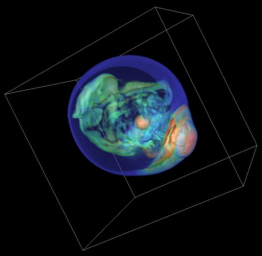
\includegraphics{VTKTextbook-104}\\
		\caption*{\texttt{Volume rendering of a supernova dataset.}}
	\end{minipage}
\end{figure}

\firstletter{C}hapter 3 introduced fundamental concepts of computer graphics.
A major topic in that chapter was how to represent and render geometry using surface primitives such as points, lines, and polygons.
In this chapter our primary focus is on volume graphics.
Compared to surface graphics, volume graphics has a greater expressive range in its ability to render inhomogeneous materials, and is a dominant technique for visualizing 3D image (volume) datasets.

We begin the chapter by describing two techniques that are important to both surface and volume graphics.
These are simulating object transparency using simple blending functions, and using texture maps to add realism without excessive computational cost.
We also describe various problems and challenges inherent to these techniques.
We then follow with a focused discussion on volume graphics, including both object-order and image-order techniques, illumination models, approaches to mixing surface and volume graphics, and methods to improve performance.
Finally, the chapter concludes with an assortment of important techniques for creating more realistic visualizations.
These techniques include stereo viewing, antialiasing, and advanced camera techniques such as motion blur, focal blur, and camera motion.

\section{Transparency and Alpha Values}
\label{sec:transparency_alpha}

Up to this point in the text we have focused on rendering opaque objects --- that is, we have assumed that objects reflect, scatter, or absorb light at their surface, and no light is transmitted through to their interior. Although rendering opaque objects is certainly useful, there are many applications that can benefit from the ability to render objects that transmit light. One important application of transparency is volume rendering, which we will explore in greater detail later in the chapter. Another simple example makes objects translucent so that we can see inside of the region bounded by the surface, as shown in Figure \ref{fig:Figure12-4}. As demonstrated in this example, by making the skin semitransparent, it becomes possible to see the internal organs.

Transparency and its complement, opacity, are often referred to as *alpha* in computer graphics. For example, a polygon that is 50 percent opaque will have an alpha value of 0.5 on a scale from zero to one. An alpha value of one represents an opaque object and zero represents a completely transparent object. Frequently, alpha is specified as a property for the entire actor, but it also can be done on a vertex basis just like colors. In such cases, the RGB specification of a color is extended to RGBA where A represents the alpha component. On many graphics cards the frame buffer can store the alpha value along with the RGB values. More typically, an application will request storage for only red, green, and blue on the graphics card and use back-to-front blending to avoid the need for storing alpha.

Unfortunately, having transparent actors introduces some complications into the rendering process. If you think back to the process of ray tracing, viewing rays are projected from the camera out into the world, where they intersect the first actor they come to. With an opaque actor, the lighting equations are applied and the resulting color is drawn to the screen. With a semitransparent actor we must solve the lighting equations for this actor, and then continue projecting the ray farther to see if it intersects any other actors. The resulting color is a composite of all the actors it has intersected. For each surface intersection this can be expressed as Equation \ref{eq:7.1}.

\begin{equation}\label{eq:7.1}
\begin{array}{lll}
R &=& (1 - A_s) R_b + A_s R_s\\
G &=& (1 - A_s) G_b + A_s G_s\\
B &=& (1 - A_s) B_b + A_s B_s\\
A &=& (1 - A_s) A_b + A_s
\end{array}
\end{equation}
\myequations{Surface interaction of colors with transparent actors.}

In this equation subscript $s$ refers to the surface of the actor, while subscript $b$ refers to what is behind the actor. The term is called the transmissivity, and represents the amount of light that is transmitted through the actor. As an example, consider starting with three polygons colored red, green, and blue each with a transparency of $0.5$. If the red polygon is in the front and the background is black, the resulting RGBA color will be $(0.4, 0.2, 0.1, 0.875)$ on a scale from zero to one (Figure \ref{fig:Figure7-1}).

\begin{figure}[!htb]
	\centering
	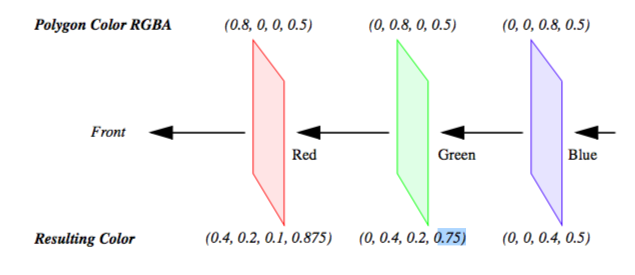
\includegraphics[width=0.8\textwidth]{Figure7-1}\\
	\caption{Alpha compositing.}\label{fig:Figure7-1}
\end{figure}

It is important to note that if we switch the ordering of the polygons, the resulting color will change. This underlies a major technical problem in using transparency. If we ray-trace a scene, we will intersect the surfaces in a well-defined manner --- from front to back. Using this knowledge we can trace a ray back to the last surface it intersects, and then composite the color by applying Equation \ref{eq:7.1} to all the surfaces in reverse order (i.e., from back to front). In object order rendering methods, this compositing is commonly supported in hardware, but unfortunately we are not guaranteed to render the polygons in any specific order. Even though our polygons are situated as in Figure \ref{fig:Figure7-1}, the order in which the polygons are rendered might be the blue polygon, followed by the red, and finally the green polygon. Consequently, the resulting color is incorrect.

If we look at the RGBA value for one pixel we can see the problem. When the blue polygon is rendered, the frame buffer and \emph{z}-buffer are empty, so the RGBA quad $(0,0,0.8,0.5)$ is stored along with the its \emph{z}-buffer value. When the red polygon is rendered, a comparison of its \emph{z}-value and the current \emph{z}-buffer indicates that it is in front of the previous pixel entry. So Equation \ref{eq:7.1} is applied using the frame buffer’s RGBA value. This results in the RGBA value $(0.4,0,0.2,0.75)$ being written to the buffer. Now, the green polygon is rendered and the z comparison indicates that it is behind the current pixel's value. Again this equation is applied, this time using the frame buffer's RGBA value for the surface and the polygon’s values from behind. This results in a final pixel color of $(0.3,0.2, 0.175,0.875)$, which is different from what we previously calculated. Once the red and blue polygons have been composited and written to the frame buffer, there is no way to insert the final green polygon into the middle where it belongs.

One solution to this problem is to sort the polygons from back to front and then render them in this order. Typically, this must be done in software requiring additional computational overhead. Sorting also interferes with actor properties (such as specular power), which are typically sent to the graphics engine just before rendering the actor's polygons. Once we start mixing up the polygons of different actors, we must make sure that the correct actor properties are set for each polygon rendered.

Another solution is to store more than one set of RGBAZ values in the frame buffer. This is costly because of the additional memory requirements, and is still limited by the number of RGBAZ values you can store. Some new techniques use a combination of multiple RGBAZ value storage and multipass rendering to yield correct results with a minimum performance hit \cite{Hodges92}.

The second technical problem with rendering transparent objects occurs less frequently, but can still have disastrous effects. In certain applications, such as volume rendering, it is desirable to have thousands of polygons with small alpha values. If the RGBA quad is stored in the frame buffer as four eight-bit values, then the round-off can accumulate over many polygons, resulting in gross errors in the output image. This may be less of a problem in the future if graphics hardware begins to store 16 or more bits per component for texture and the frame buffer.

\section{Texture Mapping}

\emph{Texture mapping} is a technique to add detail to an image without requiring modelling detail. Texture mapping can be thought of as pasting a picture to the surface of an object. The use of texture mapping requires two pieces of information: a \emph{texture map} and \emph{texture coordinates}. The texture map is the picture we paste, and the texture coordinates specify the location where the picture is pasted. More generally, texture mapping is a table lookup for color, intensity, and/or transparency that is applied to an object as it is rendered. Textures maps and coordinates are most often two-dimensional, but three-dimensional texture maps and coordinates are supported by most new graphics hardware.

The value of texture mapping can be shown through the simple example of rendering a wooden table. The basic geometry of a table can be easily created, but achieving the wood grain details is difficult. Coloring the table brown is a good start, but the image is still unrealistic. To simulate the wood grain we need to have many small color changes across the surface of the table. Using vertex colors would require us to have millions of extra vertices just to get the small color changes. The solution to this is to apply a wood grain texture map to the original polygons. This is like applying an oak veneer onto inexpensive particleboard, and this is the strategy used by video games to provide realistic scenes with low numbers of polygons for interactivity.

There are several ways in which we can apply texture data. For each pixel in the texture map (commonly called a \emph{texel} for texture element), there may be one to four components that affect how the texture map is pasted onto the surface of the underlying geometry. A texture map with one component is called an \emph{intensity map}. Applying an intensity map results in changes to the intensity (or value in HSV) of the resulting pixels. If we took a gray scale image of wood grain, and then texture-mapped it onto a brown polygon, we would have a reasonable looking table. The hue and saturation of the polygon would still be determined by the brown color, but the intensity would be determined from the texture map. A better looking table could be obtained by using a color image of the wood. This is a three component texture map, where each texel is represented as a RGB triplet. Using an RGB map allows us to obtain more realistic images, since we would have more than just the intensity changes of the wood.

By adding alpha values to an intensity map we get two components. We can do the same to an RGB texture map to get a four component RGBA texture map. In these cases, the alpha value can be used to make parts of the underlying geometry transparent. A common trick in computer graphics is to use RGBA textures to render trees. Instead of trying to model the complex geometry of a tree, we just render a rectangle with an RGBA texture map applied to it. Where there are leaves or branches, the alpha is one, where there are gaps and open space, the alpha is zero. As a result, we can see through portions of the rectangle, giving the illusion of viewing through the branches and leaves of a tree.

Besides the different ways in which a texture map can be defined, there are options in how it interacts with the original color of the object. A common option for RGB and RGBA maps is to ignore the original color; that is, just apply the texture color as specified. Another option is to modulate the original color by the texture map color (or intensity) to produce the final color.

While we have been focusing on 2D texture maps, they can be of any dimension, though the most common are 2D and 3D. Three-dimensional texture maps are used for textures that are a function of 3D space, such as wood grain, stone, or X-ray intensity (i.e., CT scan). In fact, a volumetric dataset is essentially a 3D texture. We can perform high-speed volume rendering by passing planes through a 3D texture and compositing them using translucent alpha values in the correct order.

\begin{figure}[!htb]
	\centering
	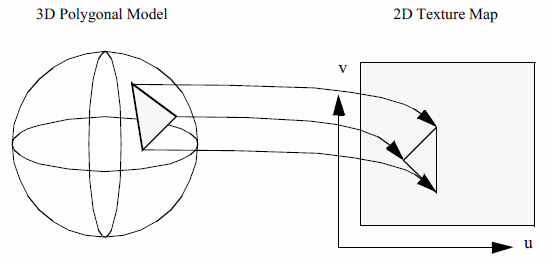
\includegraphics[width=0.8\textwidth]{Figure7-2}\\
	\caption{Vertex texture coordinates.}\label{fig:Figure7-2}
\end{figure}

Techniques for performing volume rendering using texture mapping hardware will be discussed later in this chapter.

A fundamental step in the texture mapping process is determining how to map the texture onto the geometry. To accomplish this, each vertex has an associated texture coordinate in addition to its position, surface normal, color, and other point attributes. The texture coordinate maps the vertex into the texture map as shown in Figure \ref{fig:Figure7-2}. The texture coordinate system uses the parameters $(u,v)$ and $(u,v,t)$ or equivalently ($r,s$) or ($r,s,t$) for specifying 2D and 3D texture values. Points between the vertices are linearly interpolated to determine texture map values.

Another approach to texture mapping uses procedural texture definitions instead of a texture map. In this approach, as geometry is rendered, a procedure is called for each pixel to calculate a texel value. Instead of using the $(u,v,t)$ texture coordinates to index into an image, they are passed as arguments to the procedural texture that uses them to calculate its result. This method provides almost limitless flexibility in the design of a texture; therefore, it is almost impossible to implement in dedicated hardware. Most commonly, procedural textures are used with software rendering systems that do not make heavy use of existing graphics hardware.

While texture maps are generally used to add detail to rendered images, there are important visualization applications.

\begin{itemize}

	\item Texture maps can be generated procedurally as a function of data. One example is to change the appearance of a surface based on local data value.

	\item Texture coordinates can be generated procedurally as a function of data. For example, we can threshold geometry by creating a special texture map and then setting texture coordinates based on local data value. The texture map consists of two entries: fully transparent ($\alpha = 0$) and fully opaque ($\alpha = 1$). The texture coordinate is then set to index into the transparent portion of the map if the scalar value is less than some threshold, or into the opaque portion otherwise.

	\item Texture maps can be animated as a function of time. By choosing a texture map whose intensity varies monotonically from dark to light, and then "moving" the texture along an object, the object appears to crawl in the direction of the texture map motion. We can use this technique to add apparent motion to things like hedgehogs to show vector magnitude. Figure \ref{fig:Figure7-3} is an example of a texture map animation used to simulate vector field motion.

\end{itemize}

\begin{figure}[!htb]
	\floatbox[{\capbeside\thisfloatsetup{capbesideposition={right,center},capbesidewidth=0.4\textwidth}}]{figure}[\FBwidth]
	{\caption{One frame from a vector field animation using texture.(\href{https://lorensen.github.io/VTKExamples/site/Cxx/Texture/AnimateVectors/}{AnimateVectors.cxx}) or (\href{https://lorensen.github.io/VTKExamples/site/Python/Texture/AnimateVectors/}{AnimateVectors.py})}\label{fig:Figure7-3}}
	{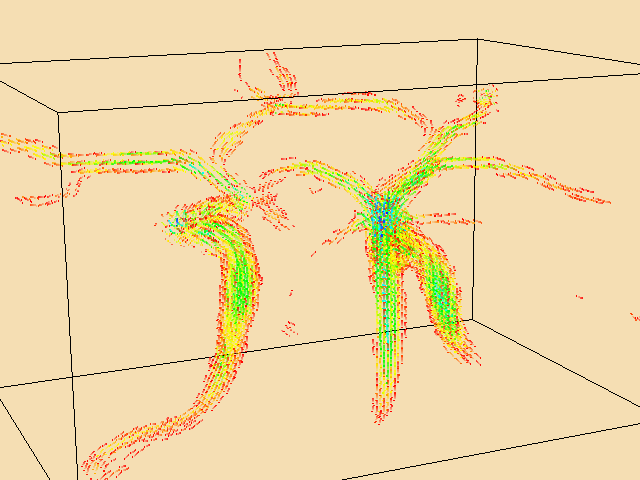
\includegraphics[width=0.6\textwidth]{Figure7-3}}
\end{figure}

These techniques will be covered in greater detail in Chapter 9: \nameref{chap:advanced_algorithms}. (See``Texture Algorithms'' on page \pageref{subsec:texture_algorithms} for more information.)

\section{Volume Rendering}
\label{sec:volume_rendering}

Until now we have concentrated on the visualization of data through the use of geometric primitives such as points, lines, and polygons.
For many applications such as architectural walk--throughs or terrain visualization, this is obviously the most efficient and effective representation for the data.
In contrast, some applications require us to visualize data that is inherently volumetric (which we refer to as 3D image or volume datasets).
For example, in biomedical imaging we may need to visualize data obtained from an MR or CT scanner, a confocal microscope, or an ultrasound study.
Weather analysis and other simulations also produce large quantities of volumetric data in three or more dimensions that require effective visualization techniques.
As a result of the popularity and usefulness of volume data over the last several decades, a broad class of rendering techniques known as volume rendering has emerged. The purpose of volume rendering is to effectively convey information within volumetric data.

In the past, researchers have attempted to define volume rendering as a process that operates directly on the dataset to produce an image without generating an intermediate geometric representation. With recent advances in graphics hardware and clever implementations, developers have been able to use geometric primitives to produce images that are identical to those generated by direct volume rendering techniques. Due to these new techniques, it is nearly impossible to define volume rendering in a manner that is clearly distinct from geometric rendering. Therefore, we choose a broad definition of volume rendering as any method that operates on volumetric data to produce an image.

The next several sections cover a variety of volume rendering methods that use direct rendering techniques, geometric primitive rendering techniques, or a combination of these two methods, to produce an image. Some of the direct volume rendering techniques discussed in this chapter generate images that are nearly identical to those produced by geometric rendering techniques discussed in earlier chapters. For example, using a ray casting method to produce an isosurface image is similar, though not truly equivalent, to rendering geometric primitives that were extracted with the marching cubes contouring technique described in Chapter 6.

The two basic surface rendering approaches described in Chapter 3, image-order and object-order, apply to volume rendering techniques as well. In an image-order method, rays are cast for each pixel in the image plane through the volume to compute pixel values, while in an object--order method the volume is traversed, typically in a front--to--back or back--to--front order, with each voxel processed to determine its contribution to the image. In addition, there are other volume rendering techniques that cannot easily be classified as image-order or object--order. For example, a volume rendering technique may traverse both the image and the volume simultaneously, or the image may be computed in the frequency domain rather than the spatial domain.

Since volume rendering is typically used to generate images that represent an entire 3D dataset in a 2D image, several new challenges are introduced. Classification must be performed to assign color and opacity to regions within the volume, and volumetric illumination models must be defined to support shading. Furthermore, efficiency and compactness are of great importance due to the complexity of volume rendering methods and the size of typical volumetric datasets. A geometric model that consists of one million primitives is generally considered large, while a volumetric dataset with one million voxels is quite small. Typical volumes contain between ten and several hundred million voxels, with datasets of a billion or more voxels becoming more common. Clearly care must be taken when deciding to store auxiliary information at each voxel or to increase the time required to process each voxel.

\section{Image-Order Volume Rendering}

Image-order volume rendering is often referred to as ray casting or ray tracing. The basic idea is that we determine the value of each pixel in the image by sending a ray through the pixel into the scene according to the current camera parameters. We then evaluate the data encountered along the ray using some specified function in order to compute the pixel value. As we will demonstrate throughout this chapter, ray casting is a flexible technique that can be used to render any 3D image dataset, and can produce a variety images. Also, it is relatively easy to extend a basic ray casting technique designed for volumetric data sets that have uniform voxels to work on rectilinear or structured grids. Unfortunately, basic ray casting is also fairly slow; therefore, later in this chapter we will discuss a number of acceleration methods that can be used to improve performance, though often with some additional memory requirements or loss in flexibility.

\begin{figure}[!htb]
	\floatbox[{\capbeside\thisfloatsetup{capbesideposition={left,center},capbesidewidth=0.4\textwidth}}]{figure}[\FBwidth]
	{\caption{A maximum intensity projection created with a ray casting technique. Intensity values are mapped through the color lookup table shown at the bottom of the image before display.}\label{fig:Figure7-4}}
	{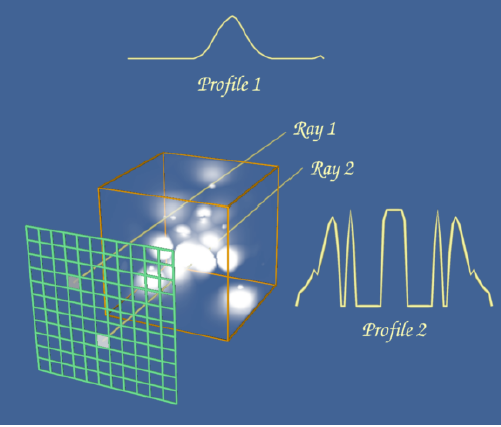
\includegraphics[width=0.6\textwidth]{Figure7-4}}
\end{figure}


The ray casting process is illustrated in Figure \ref{fig:Figure7-4}. This example uses a standard orthographic camera projection; consequently, all rays are parallel to each other and perpendicular to the view plane. The data values along each ray are processed according to the ray function, which in this case determines the maximum value along the ray and converts it to a gray scale pixel value where the minimum scalar value in the volume maps to transparent black, and the maximum scalar value maps to opaque white.

The two main steps of ray casting are determining the values encountered along the ray, and then processing these values according to a ray function. Although in implementation these two steps are typically combined, we will treat them independently for the moment. Since the specific ray function often determines the method used to extract values along the ray, we will begin by considering some of the basic ray function types.

\begin{figure}[!htb]
	\begin{subfigure}[h]{0.96\linewidth}
		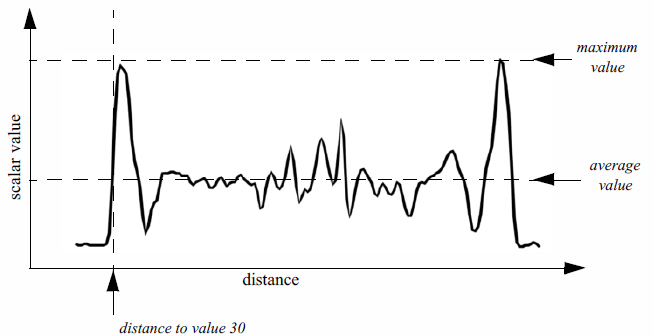
\includegraphics[width=\linewidth]{Figure7-5a}
		\caption*{}\label{fig:Figure7-5a}
	\end{subfigure}
	\hfill
	\begin{subfigure}[h]{0.48\linewidth}
		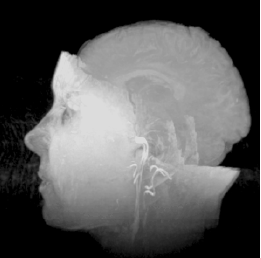
\includegraphics[width=\linewidth]{Figure7-5b}
		\caption*{Maximum value}\label{fig:Figure7-5b}
	\end{subfigure}%
	\hfill
	\begin{subfigure}[h]{0.48\linewidth}
		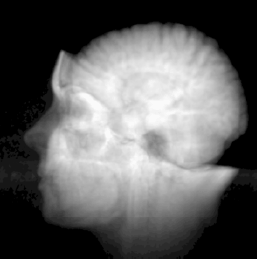
\includegraphics[width=\linewidth]{Figure7-5c}
		\caption*{Average value}\label{fig:Figure7-5c}
	\end{subfigure}
	\hfill
	\begin{subfigure}[h]{0.48\linewidth}
		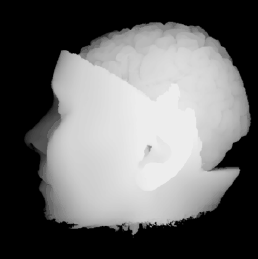
\includegraphics[width=\linewidth]{Figure7-5d}
		\caption*{Distance to value 30}\label{fig:Figure7-5d}
	\end{subfigure}%
	\hfill
	\begin{subfigure}[h]{0.48\linewidth}
		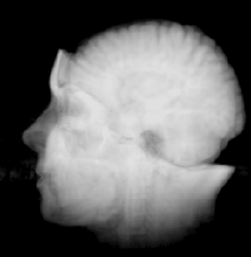
\includegraphics[width=\linewidth]{Figure7-5e}
		\caption*{Composite}\label{fig:Figure7-5e}
	\end{subfigure}
	\caption{A ray profile and four example ray functions. MRI head data courtesy of Siemens Medical Systems, Inc., Iselin, NJ.}\label{fig:Figure7-5}
\end{figure}

Figure \ref{fig:Figure7-5} shows the data value profile of a ray as it passes through 8 bit volumetric data where the data values can range between 0 and 255. The \emph{x}-axis of the profile indicates distance from the view plane while the \emph{y}-axis represents data value. The results obtained from four different simple ray functions are shown below the profile. For display purposes we convert the raw result values to gray scale values using a method similar to the one in the previous example.

The first two ray functions, maximum value and average value, are basic operations on the scalar values themselves. The third ray function computes the distance along the ray at which a scalar value at or above 30 is first encountered, while the fourth uses an alpha compositing technique, treating the values along the ray as samples of opacity accumulated per unit distance. Unlike the first three ray functions, the result of the compositing technique is not a scalar value or distance that can be represented on the ray profile.

\begin{figure}[!htb]
	\centering
	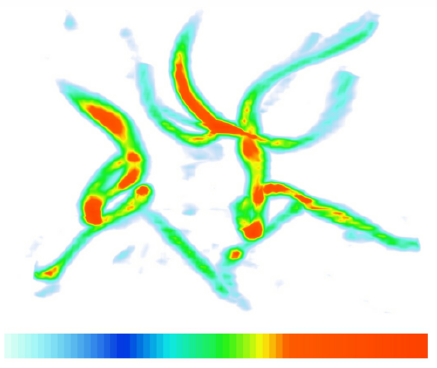
\includegraphics[width=0.8\textwidth]{Figure7-6}\\
	\caption{Image-order volume rendering. High potential iron protein data courtesy of Scripps Clinic, La Jolla, CA.}\label{fig:Figure7-6}
\end{figure}

The maximum intensity projection, or MIP, is probably the simplest way to visualize volumetric data. This technique is fairly forgiving when it comes to noisy data, and produces images that provide an intuitive understanding of the underlying data. One problem with this method is that it is not possible to tell from a still image where the maximum value occurred along the ray. For example, consider the image of a carotid artery shown in Figure \ref{fig:Figure7-6}. We are unable to fully understand the structure of the blood vessels from this still image since we cannot determine whether some vessel is in front of or behind some other vessel. This problem can be solved by generating a small sequence of images showing the data rotating, although for parallel camera projections even this animation will be ambiguous. This is due to the fact that two images generated from cameras that view the data from opposite directions will be identical except for a reflection about the Y axis of the image.

\begin{figure}[!htb]
	\begin{subfigure}[h]{0.48\linewidth}
		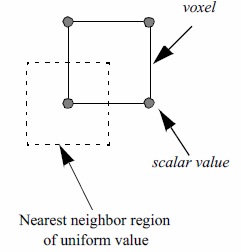
\includegraphics[width=\linewidth]{Figure7-7a}
		\caption*{}\label{fig:Figure7-7a}
	\end{subfigure}
	\hfill
	\begin{subfigure}[h]{0.48\linewidth}
		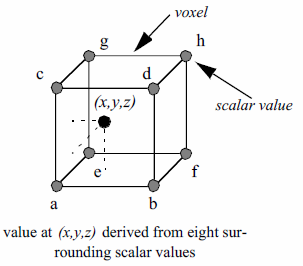
\includegraphics[width=\linewidth]{Figure7-7b}
		\caption*{}\label{fig:Figure7-7b}
	\end{subfigure}%
	\caption{A 2D example of nearest neighbor interpolation (left) and a 3D example of trilinear interpolation (right).}\label{fig:Figure7-7}
\end{figure}

Later in this chapter, during the classification and illumination discussions, we will consider more complex ray functions. Although the colorful, shaded images produced by the new methods may contain more information, they may also be more difficult to interpret, and often easier to misinterpret, than the simple images of the previous examples. For that reason, it is beneficial to use multiple techniques to visualize your volumetric data.

A volume is represented as a 3D image dataset where scalar values are defined at the points of the regular grid, yet in ray casting we often need to sample the volume at arbitrary locations. To do this we must define an interpolation function that can return a scalar value for any location between grid points. The simplest interpolation function, which is called zero-order, constant, or nearest neighbor interpolation, returns the value of the closest grid point. This function defines a grid of identical rectangular boxes of uniform value centered on grid points, as illustrated in 2D on the left side of Figure \ref{fig:Figure7-7}. In the image on the right we see an example of trilinear interpolation where the value at some location is defined by using linear interpolation based on distance along each of the three axes. In general, we refer to the region defined by eight neighboring grid points as a voxel. In the special case where a discrete algorithm is used in conjunction with nearest neighbor interpolation, we may instead refer to the constant-valued regions as voxels.

\begin{figure}[!htb]
	\begin{subfigure}[h]{0.48\linewidth}
		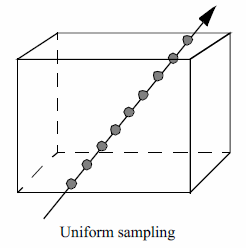
\includegraphics[width=\linewidth]{Figure7-8a}
		\caption*{}\label{fig:Figure7-8a}
	\end{subfigure}
	\hfill
	\begin{subfigure}[h]{0.48\linewidth}
		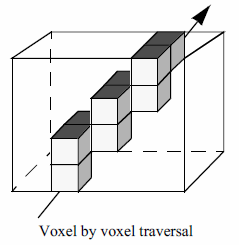
\includegraphics[width=\linewidth]{Figure7-8b}
		\caption*{}\label{fig:Figure7-8b}
	\end{subfigure}%
	\caption{Two basic ray traversal methods for volume rendering.}\label{fig:Figure7-8}
\end{figure}

To traverse the data along a ray, we could sample the volume at uniform intervals or we could traverse a discrete representation of the ray through the volume, examining each voxel encountered, as illustrated in Figure \ref{fig:Figure7-8}. The selection of a method depends upon factors such as the interpolation technique, the ray function, and the desired trade-off between image accuracy and speed.

The ray is typically represented in parametric form as

\begin{equation}\label{eq:7.2}
\left(x, y, z\right) = \left(x_0, y_0, z_0\right) + \left(a, b, c\right) t
\end{equation}
\myequations{Parametric equation of a ray.}

where $x_0,y_0,z_0)$ is the origin of the ray (either the camera position for
perspective viewing transformations or a pixel on the view plane for parallel viewing transformations), and $(a, b, c)$ is the normalized ray direction vector. If t1 and t2 represent the distances where the ray enters and exits the volume respectively, and delta\_t indicates the step size, then we can use the following code fragment to perform uniform distance sampling:

\begin{lstlisting}[language=C++, caption={Uniform distance sampling.}]
t = t1;
v = undefined;
while ( t < t2 )
  {
  x = x0 + a * t;
  y = y0 + b * t;
  z = z0 + c * t;
  v = EvaluateRayFunction( v, t );
  t = t + delta_t;
  }
\end{lstlisting}

\begin{figure}[!htb]
	\begin{subfigure}[h]{0.32\linewidth}
		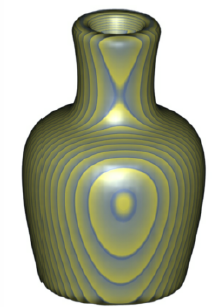
\includegraphics[width=\linewidth]{Figure7-9a}
		\caption*{Step size = 2.0}\label{fig:Figure7-9a}
	\end{subfigure}
	\hfill
	\begin{subfigure}[h]{0.32\linewidth}
		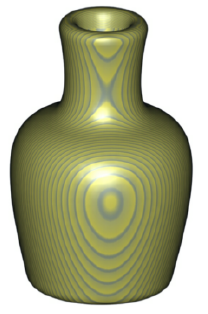
\includegraphics[width=\linewidth]{Figure7-9b}
		\caption*{Step size = 1.0}\label{fig:Figure7-9b}
	\end{subfigure}%
	\hfill
	\begin{subfigure}[h]{0.32\linewidth}
		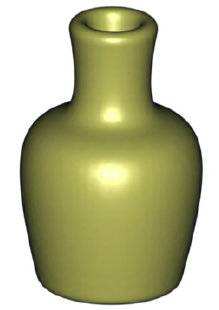
\includegraphics[width=\linewidth]{Figure7-9c}
		\caption*{Step size = 0.1}\label{fig:Figure7-9c}
	\end{subfigure}%
	\caption{Images generated using a ray casting method with three different step sizes.Vase data courtesy of SUNY Stony Brook.}\label{fig:Figure7-9}
\end{figure}

One difficulty with the uniform distance sampling method is selecting the step size. If the step size is too large, then our sampling might miss features in the data, yet if we select a small step size, we will significantly increase the amount of time required to render the image. This problem is illustrated in Figure \ref{fig:Figure7-9} using a volumetric dataset with grid points that are one unit apart along the X, Y, and Z axes. The images were generated using step sizes of 2.0, 1.0, and 0.1 units, where the 0.1 step-size image took nearly 10 times as long to generate as the 1.0 step-size image, which in turn took twice as long to render as the 2.0 step-size image. A compositing method was used to generate the images, where the scalar values within the dataset transition sharply from transparent black to opaque white. If the step size is too large, a banding effect appears in the image highlighting regions of the volume equidistant from the ray origin along the viewing rays. To reduce this effect when a larger step size is desired for performance reasons, the origin of each ray can be bumped forward along the viewing direction by some small random offset, which will produce a more pleasing image by eliminating the regular pattern of the aliasing.

In some cases it may make more sense to examine each voxel along the ray rather than taking samples. For example, if we are visualizing our data using a nearest neighbor interpolation method, then we may be able to implement a more efficient algorithm using discrete ray traversal and integer arithmetic. Another reason for examining voxels may be to obtain better accuracy on certain ray functions. We can compute the exact maximum value encountered along a ray within each voxel when using trilinear interpolation by taking the first derivative of the interpolation function along the ray and solving the resulting equation to compute the extrema. Similarly, we can find the exact location along the ray where a selected value is first encountered to produce better images of isovalue surfaces within the volume.

\begin{figure}[!htb]
	\begin{subfigure}[h]{0.24\linewidth}
		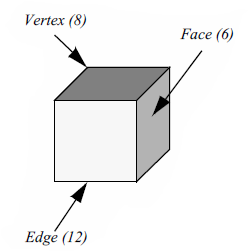
\includegraphics[width=\linewidth]{Figure7-10a}
		\caption*{}\label{fig:Figure7-10a}
	\end{subfigure}
	\hfill
	\begin{subfigure}[h]{0.24\linewidth}
		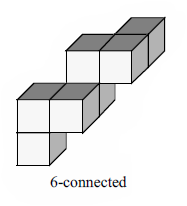
\includegraphics[width=\linewidth]{Figure7-10b}
		\caption*{}\label{fig:Figure7-10b}
	\end{subfigure}%
	\hfill
	\begin{subfigure}[h]{0.24\linewidth}
		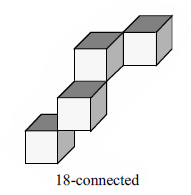
\includegraphics[width=\linewidth]{Figure7-10c}
		\caption*{}\label{fig:Figure7-10c}
	\end{subfigure}%
	\hfill
	\begin{subfigure}[h]{0.24\linewidth}
		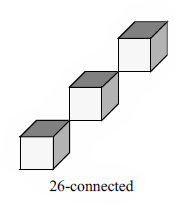
\includegraphics[width=\linewidth]{Figure7-10d}
		\caption*{}\label{fig:Figure7-10d}
	\end{subfigure}%
	\caption{Discrete ray classification.}\label{fig:Figure7-10}
\end{figure}

A 3D scan conversion technique, such as a modified Bresenham method, can be used to transform the continuous ray into a discrete representation. The discrete ray is an ordered sequence of voxels $v_1, v_2,... v_n$ and can be classified as 6-connected, 18-connected, or 26-connected as shown in Figure \ref{fig:Figure7-10}. Each voxel contains 6 faces, 12 edges, and 8 vertices. If each pair of voxels  $v_i, v_{i+1}$ along the ray share a face then the ray is 6-connected, if they share a face or an edge the ray is 18-connected, and if they share a face, an edge, or a vertex the ray is 26-connected. Scan converting and traversing a 26-connected ray requires less time than a 6-connected ray but is more likely to miss small features in the volume dataset.

\begin{figure}[!htb]
	\begin{subfigure}[h]{0.48\linewidth}
		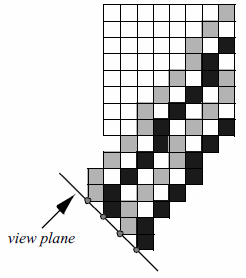
\includegraphics[width=\linewidth]{Figure7-11a}
		\caption*{}\label{fig:Figure7-11a}
	\end{subfigure}
	\hfill
	\begin{subfigure}[h]{0.48\linewidth}
		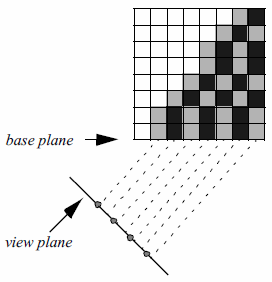
\includegraphics[width=\linewidth]{Figure7-11b}
		\caption*{}\label{fig:Figure7-11b}
	\end{subfigure}%
	\caption{Ray casting with templated discrete rays. If the rays originate from the image plane (left) then voxels are missed in the volume. If instead the rays originate from a base plane of the volume (right), each voxel is visited exactly once.}\label{fig:Figure7-11}
\end{figure}

If we are using a parallel viewing transformation and our ray function can be efficiently computed using a voxel by voxel traversal method, then we can employ a templated ray casting technique \cite{Yagel92b} with 26-connected rays to generate the image. All rays are identical in direction; therefore, we only need to scan convert once, using this "template" for every ray. When these rays are cast from pixels on the image plane, as shown in the left image of Figure \ref{fig:Figure7-11}, then some voxels in the dataset will not contribute to the image. If instead we cast the rays from the voxels in the base plane of the volume that is most parallel to the image plane, as shown in the right image, then the rays fit together snugly such that every voxel in the dataset is visited exactly once. The image will appear warped because it is generated from the base plane, so a final resampling step is required to project this image back onto the image plane.

\section{Object-Order Volume Rendering}

Object-order volume rendering methods process samples in the volume based on the organization of the voxels in the dataset and the current camera parameters. When an alpha compositing method is used, the voxels must be traversed in either a front-to-back or back-to-front order to obtain correct results. This process is analogous to sorting translucent polygons before each projection in order to ensure correct blending. When graphics hardware is employed for compositing, a back-to-front ordering is typically preferred since it is then possible to perform alpha blending without the need for alpha bitplanes in the frame buffer. If a software compositing method is used, a front-to-back ordering is more common since partial image results are more visually meaningful, and can be used to avoid additional processing when a pixel reaches full opacity. Voxel ordering based on distance to the view plane is not always necessary since some volume rendering operations, such as MIP or average, can be processed in any order and still yield correct results.

\begin{figure}[!htb]
	\floatbox[{\capbeside\thisfloatsetup{capbesideposition={left,center},capbesidewidth=0.4\textwidth}}]{figure}[\FBwidth]
	{\caption{Object-order, back-to-front volume rendering.}\label{fig:Figure7-12}}
	{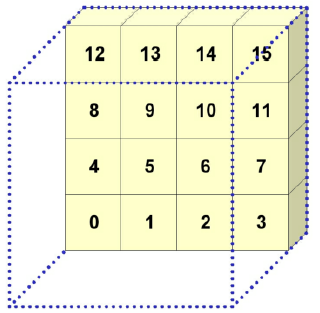
\includegraphics[width=0.6\textwidth]{Figure7-12}}
\end{figure}

Figure ref{Figure7-12} illustrates a simple object-order, back-to-front approach to projecting the voxels in a volume for an orthographic projection. Voxel traversal starts at the voxel that is furthest from the view plane and then continues progressively to closer voxels until all voxels have been visited. This is done within a triple nested loop where, from the outer to the inner loop, the planes in the volume are traversed, the rows in a plane are processed, and finally the voxels along a row are visited. Figure ref{Figure7-12} shows an ordered labeling of the first seven voxels as the volume is projected. Processing voxels in this manner does not yield a strict ordering from the furthest to the closest voxel. However, it is sufficient for orthographic projections since it does ensure that the voxels that project to a single pixel are processed in the correct order.

\begin{figure}[!htb]
	\floatbox[{\capbeside\thisfloatsetup{capbesideposition={right,center},capbesidewidth=0.4\textwidth}}]{figure}[\FBwidth]
	{\caption{A Gaussian kernel is projected onto the view plane to produce a splat footprint.}\label{fig:Figure7-13}}
	{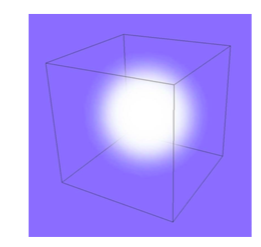
\includegraphics[width=0.6\textwidth]{Figure7-13}}
\end{figure}

When a voxel is processed, its projected position on the view plane is determined and an operation is performed at that pixel location using the voxel and image information. This operator is similar to the ray function used in image-order ray casting techniques. Although this approach to projecting voxels is both fast and efficient, it often yields image artifacts due to the discrete selection of the projected image pixel. For instance, as we move the camera closer to the volume in a perspective projection, neighboring voxels will project to increasingly distant pixels on the view plane, resulting in distracting "holes" in the image.

A volume rendering technique, called splatting, addresses this problem by distributing the energy of a voxel across many pixels. Splatting is an object-order volume rendering technique proposed by Westover \cite{Westover90} and, as its name implies, it projects the energy of a voxel onto the image plane one splat, or footprint, at a time. A kernel with finite extent is placed around each data sample. The footprint is the projected contribution of this sample onto the image plane, and is computed by integrating the kernel along the viewing direction and storing the results in a 2D footprint table. Figure ref{Figure7-13} illustrates the projection of a Gaussian kernel onto the image plane that may then be used as a splatting footprint. For a parallel viewing transform and a spherically symmetric kernel, the footprint of every voxel is identical except for an image space offset. Therefore, the evaluation of the footprint table and the image space extent of a sample can be performed once as a preprocessing step to volume rendering. Splatting is more difficult for perspective volume rendering since the image space extent is not identical for all samples. Accurately correcting for perspective effects in a splatting approach would make the algorithm far less efficient. However, with a small loss of accuracy we can still use the generic footprint table if we approximate the image plane extent of an ellipsoid with an ellipse.

There are several important considerations when utilizing a splatting approach for volume rendering. The type of kernel, the radius of the kernel, and the resolution of the footprint table will all impact the appearance of the final image. For example, a kernel radius that is smaller than the distance between neighboring samples may lead to gaps in the image, while a larger radius will lead to a blurry image. Also, a low resolution footprint table is faster to precompute, but a high resolution table allows us to use nearest neighbor sampling for faster rendering times without a significant loss in image accuracy.

\begin{figure}[!htb]
	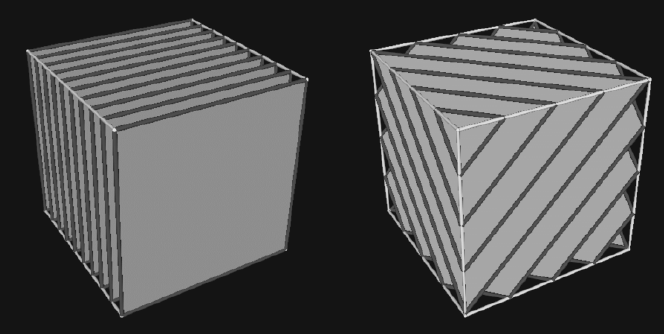
\includegraphics[width=0.96\linewidth]{Figure7-14}
	\caption{Volume rendering using a 2D (left) and 3D (right) texture mapping technique.}\label{fig:Figure7-14}
\end{figure}

Texture mapping as described earlier in this chapter was originally developed to provide the appearance of high surface complexity when rendering geometric surfaces. As texture mapping methods matured and found their way into standard graphics hardware, researchers began utilizing these new capabilities to perform volume rendering \cite{Cabral94}. There are two main texture-mapped volume rendering techniques based on the two main types of texture hardware currently available. Two-dimensional texture-mapped volume rendering makes use of 2D texture mapping hardware whereas 3D texture-mapped volume rendering makes use less commonly available 3D texture mapping graphics hardware.

We can decompose texture-mapped volume rendering into two basic steps. The first is a sampling step where the data samples are extracted from the volume using some form of interpolation. Depending on the type of texture hardware available, this may be nearest neighbor, bilinear, or tri-linear interpolation and may be performed exclusively in hardware or through a combination of both software and hardware techniques. The second step is a blending step where the sampled values are combined with the current image in the frame buffer. This may be a simple maximum operator or it may be a more complex alpha compositing operator.

Texture-mapped volume renderers sample and blend a volume to produce an image by projecting a set of texture-mapped polygons that span the entire volume. In 2D texture-mapped volume rendering the dataset is decomposed into a set of orthographic slices along the axis of the volume most parallel to the viewing direction. The basic rendering algorithm consists of a loop over the orthogonal slices in a back-to-front order, where for each slice, a 2D texture is downloaded into texture memory. Each slice, which is a rectangular polygon, is projected to show the entire 2D texture. If neighboring slices are far apart relative to the image size, then it may be necessary to use a software bilinear interpolation method to extract additional slices from the volume in order to achieve a desired image accuracy. The image on the left side of Figure \ref{fig:Figure7-14} illustrates the orthogonal slices that are rendered using a 2D texture mapping approach. Several example images generated using 2D texture-mapped volume rendering are shown in Figure \ref{fig:Figure7-15}.

\begin{figure}[!htb]
	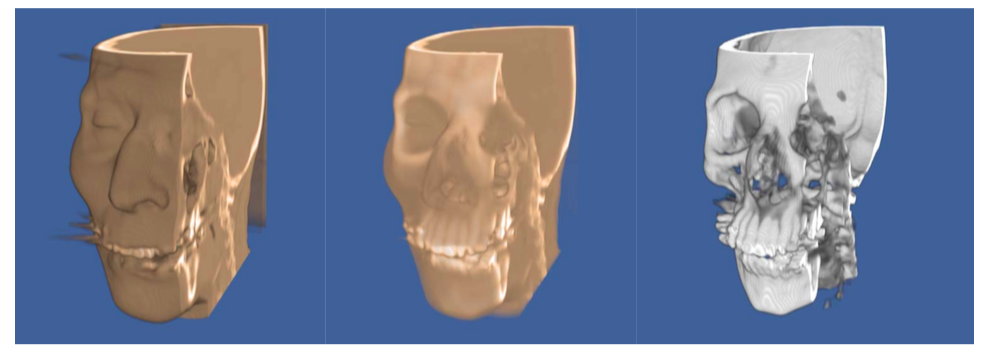
\includegraphics[width=0.96\linewidth]{Figure7-15}
	\caption{2D texture-mapped volume rendering. The images were generated using three different mappings of scalar value to opacity. CT data $(256 \times 256 \times 225)$ courtesy of North Carolina Memorial Hospital.}\label{fig:Figure7-15}
\end{figure}

The performance of this algorithm can be decomposed into the software sampling rate, the texture download rate, and the texture-mapped polygon scan conversion rate. The software sampling step is required to create the texture image, and is typically dependent on view direction due to cache locality when accessing volumetric data stored in a linear array. Some implementations minimize the software sampling cost at the expense of memory by precomputing and saving images for the three major volume orientations. The texture download rate is the rate at which this image can be transferred from main memory to texture mapping memory. The scan conversion of the polygon is usually limited by the rate at which the graphics hardware can process pixels in the image, or the pixel fill rate. For a given hardware implementation, the download time for a volume is fixed and will not change based on viewing parameters. However, reducing the relative size of the projected volume will reduce the number of samples processed by the graphics hardware that, in turn, will increase volume rendering rates at the expense of image quality.

Unlike 2D hardware, 3D texture hardware is capable of loading and interpolating between multiple slices in a volume by utilizing 3D interpolation techniques such as trilinear interpolation. If the texture memory is large enough to hold the entire volume, then the rendering algorithm is simple. The entire volume is downloaded into texture memory once as a preprocessing step. To render an image, a set of equally spaced planes along the viewing direction and parallel to the image plane is clipped against the volume. The resulting polygons, illustrated in the image on the right side of Figure \ref{fig:Figure7-14}, are then projected in back-to-front order with the appropriate 3D texture coordinates.

For large volumes it may not be possible to load the entire volume into 3D texture memory. The solution to this problem is to break the dataset into small enough subvolumes, or bricks, so that each brick will fit in texture memory. The bricks must then be processed in back-to-front order while computing the appropriately clipped polygon vertices inside the bricks. Special care must be taken to ensure that boundaries between bricks do not result in image artifacts.

Similar to a 2D texture mapping method, the 3D algorithm is limited by both the texture download and pixel fill rates of the machine. However, 3D texture mapping is superior to the 2D version in its ability to sample the volume, generally yielding higher quality images with fewer artifacts. Since it is capable of performing trilinear interpolation, we are able to sample at any location within the volume. For instance, a 3D texture mapping algorithm can sample along polygons representing concentric spheres rather than the more common view-aligned planes.

In theory, a 3D texture-mapped volume renderer and a ray casting volume renderer perform the same computations, have the same complexity, $O(n^3)$, and produce identical images. Both sample the entire volume using either nearest neighbor or trilinear interpolation, and combine the samples to form a pixel value using, for example, a maximum value or compositing function. Therefore, we can view 3D texture mapping and standard ray casting methods as functionally equivalent. The main advantage to using a texture mapping approach is the ability to utilize relatively fast graphics hardware to perform the sampling and blending operations. However, there are currently several drawbacks to using graphics hardware for volume rendering. Hardware texture-mapped volume renderings tend to have more artifacts than software ray casting techniques due to limited precision within the frame buffer for storing partial results at each pixel during blending. In addition, only a few ray functions are supported by the hardware, and advanced techniques such as shading are more difficult to achieve. However, these limitations are beginning to disappear as tex-ture mapping hardware evolves. Through the use of extensions to the OpenGL standard, per pixel vectors can be defined allowing for hardware shaded volume texture mapping. Other extensions have allowed for maximum intensity projections, and deeper framebuffers eliminate artifacts.

\section{Other Volume Rendering Methods}

\begin{figure}[!htb]
	\begin{subfigure}[h]{0.48\linewidth}
		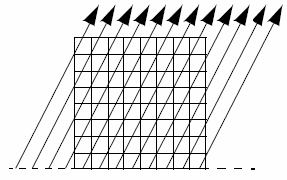
\includegraphics[width=\linewidth]{Figure7-16a}
		\caption*{}\label{fig:Figure7-16a}
	\end{subfigure}
	\hfill
	\begin{subfigure}[h]{0.48\linewidth}
		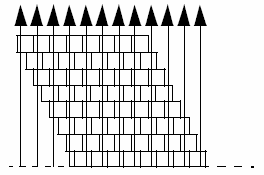
\includegraphics[width=\linewidth]{Figure7-16b}
		\caption*{}\label{fig:Figure7-16b}
	\end{subfigure}%
	\caption{On the left, orthographic rays are cast from the base plane of the volume. In the right image the volume is sheared such that these rays become perpendicular to the base plane.}\label{fig:Figure7-16}
\end{figure}

Not all volume rendering methods fall cleanly into the image-order or object-order categories. For example, the shear-warp method \cite{Lacroute94} of volume rendering traverses both image and object space at the same time. The basic idea behind this method is similar to that of templated ray casting. If we cast rays from the base plane of the volume for an orthographic projection, then it is possible to shear the volume such that the rays become perpendicular to the base plane, as shown in Figure \ref{fig:Figure7-16}. Looking at the problem this way, it is clear to see that if all rays originate from the same place within the voxels on the base plane, then these rays intersect the voxels on each subsequent plane of the volume at consistent locations. Using bilinear interpolation on the 2D planes of the dataset, we can precompute one set of interpolation weights for each plane. Instead of traversing the volume by evaluating samples along each ray, an object-order traversal method can be used to visit voxels along each row in each plane in a front-to-back order through the volume. There is a one-to-one correspondence between samples in a plane of the volume and pixels on the image plane, making it possible to traverse both the samples and the pixels simultaneously. As in templated ray casting, a final resampling (warping) operation must be performed to transform the image from sheared space on the base plane to cartesian space on the image plane.

Shear-warp volume rendering is essentially an efficient variant of ray casting. The correspondence between samples and pixels allows us to take advantage of a standard ray casting technique known as early ray termination. When we have determined that a pixel has reached full opacity during compositing, we no longer need to consider the remaining samples that project onto this pixel since they do not contribute to the final pixel value. The biggest efficiency improvement in shear-warp volume rendering comes from run-length encoding the volume. This compression method removes all empty voxels from the dataset, leaving only voxels that can potentially contribute to the image. Depending on the classification of the data, it is possible to achieve a greater than 10:1 reduction in voxels. As we step through the compressed volume, the number of voxels skipped due to run-length encoding also indicates the number of pixels to skip in the image. One drawback to this method is that it requires three copies of the compressed volume to allow for front-to-back traversal from all view directions. In addition, if we wish to use a perspective viewing transformation then we may need to traverse all three compressed copies of the volume in order to achieve the correct traversal order.

Volume rendering can also be performed using the Fourier slice projection theorem \cite{Totsuka92} that states that if we extract a slice of the volume in the frequency domain that contains the center and is parallel to the image plane, then the 2D spectrum of that slice is equivalent to the 2D image obtained by taking line integrals through the volume from the pixels on the image plane. Therefore we can volume render the dataset by extracting the appropriate slice from the 3D Fourier volume, then computing the 2D inverse Fourier transform of this slice. This allows us to render the image in $O(n^2log\ n)$ time as opposed to the $O(n^3)$ complexity required by most other volume rendering algorithms.

Two problems that must be addressed when implementing a frequency domain volume renderer are the high cost of interpolation when extracting a slice from the Fourier volume, and the high memory requirements (usually two double precision floating-point values per sample) required to store the Fourier volume. Although some shading and depth cues can be provided with this method, occlusion is not possible.

\section{Volume Classification}

\begin{figure}[!htb]
	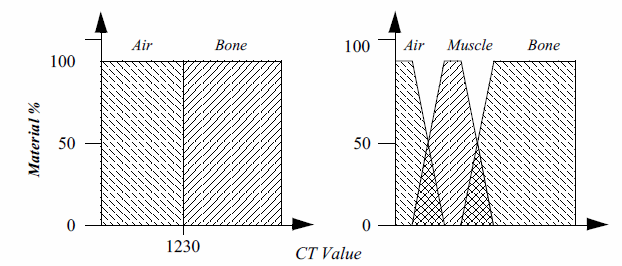
\includegraphics[width=0.96\linewidth]{Figure7-17}
	\caption{Transfer functions that classify CT densities into material percentages. A simple binary classification used to define a bone isosurface (left) and a gradual transition from air to muscle to bone (right) is shown.}\label{fig:Figure7-17}
\end{figure}

Classifying the relevant objects of interest within a dataset is a critical step in producing a volume rendered image. This information is used to determine the contribution of an object to the image as well as the object's material properties and appearance. For example, a simple binary classification of whether a data sample corresponds to bone within a CT dataset is often performed by specifying a density threshold. When the scalar value at a voxel is greater than this threshold, it is classified as bone, otherwise it is considered air. This essentially specifies an isosurface in the volume at the transition between air and bone. If we plot this operation over all possible scalar values we will get the binary step function shown on the left in Figure \ref{fig:Figure7-17}. In volume rendering we refer to this function as a transfer function. A transfer function is responsible for mapping the information at a voxel location into different values such as material, color, or opacity. The strength of volume rendering is that it can handle transfer functions of much greater complexity than a binary step function. This is often necessary since datasets contain multiple materials and classification methods cannot always assign a single material to a sample with 100 percent probability. Using advanced image segmentation and classification techniques, the single component volume can be processed into multiple material percentage volumes cite{Drebin88}. Referring back to our CT example, we can now specify a material percentage transfer function that defines a gradual transition from air to muscle, then from muscle to bone, as shown on the right in Figure \ref{fig:Figure7-17}.

\begin{figure}[!htb]
	\floatbox[{\capbeside\thisfloatsetup{capbesideposition={right,center},capbesidewidth=0.4\textwidth}}]{figure}[\FBwidth]
	{\caption{Volume rendering using a gradient magnitude opacity transfer function. Rendering performed with Kitware's VolView volume rendering system. The Visible Man CT data is courtesy of The National Library of Medicine}\label{fig:Figure7-18}}
	{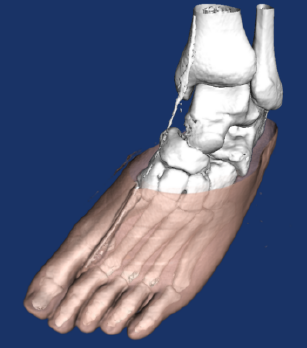
\includegraphics[width=0.6\textwidth]{Figure7-18}}
\end{figure}

In addition to material percentage transfer functions, we can define four independent transfer functions that map scalar values into red, green, blue, and opacity values for each material in the dataset. For simplicity, these sets of transfer functions are typically preprocessed into one function each for red, green, blue and opacity at the end of the classification phase. During rendering we must decide how to perform interpolation to compute the opacity and color at an arbitrary location in the volume. We could interpolate scalar value then evaluate the transfer functions, or we could evaluate the transfer functions at the grid points then interpolate the resulting opacities and colors. These two methods will produce different image results. It is generally considered more accurate to classify at the grid points then interpolate to obtain color and opacity; although if we interpolate then classify, the image often appears more pleasing since high frequencies may be removed by the interpolation.

Classifying a volume based on scalar value alone is often not capable of isolating an object of interest. A technique introduced by Levoy \cite{Levoy88} adds a gradient magnitude dimension to the specification of a transfer function. With this technique we can specify an object in the volume based on a combination of scalar value and the gradient magnitude. This allows us to define an opacity transfer function that can target voxels with scalar values in a range of densities and gradients within a range of gradient magnitudes. This is useful for avoiding the selection of homogeneous regions in a volume and highlighting fast-changing regions. Figure \ref{fig:Figure7-18} shows a CT scan of a human foot. The sharp changes in the volume, such as the transition from air to skin and flesh to bone, are shown. However, the homogeneous regions, such as the internal muscle, are mostly transparent.

If we are using a higher-order interpolation function such as tri-cubic interpolation then we can analytically compute the gradient vector at any location in the dataset by evaluating the first derivative of the interpolation function. Although we can use this approach for trilinear interpolation, it may produce undesirable artifacts since trilinear interpolation is not continuous in its first derivative across voxel boundaries. An alternative approach is to employ a finite differences technique to approximate the gradient vector:

\begin{equation}\label{eq:7.3}
\begin{array}{lll}
g_x &=& \dfrac{f(x + \Delta x, y, z) - f(x - \Delta x, y, z)}{2 \Delta x} \\ \\
g_y &=& \dfrac{f(x, y + \Delta y, z) - f(x, y - \Delta y, z)}{2 \Delta y} \\ \\
g_z &=& \dfrac{f(x, y, z + \Delta z) - f(x, y, z - \Delta z)}{2 \Delta z}
\end{array}
\end{equation}
\myequations{Finite difference approximation of a gradient vector.}

where $f(x,y,z)$ represents the scalar value at $(x,y,z)$ location in the dataset according to the interpolation function, and $g_x, g_y$ and $g_z$ are the partial derivatives of this function along the x, y, and z axes respectively. The magnitude of the gradient at $(x,y,z)$ is the length of the resulting vector $(g_x, g_y, g_z)$. This vector can also be normalized to produce a unit normal vector. The  $\Delta x, \Delta y, $ and $\Delta z$ are critical as shown in Figure \ref{fig:Figure7-19}. If these values are too small, then  the gradient vector field derived from Equation \ref{eq:7.3} may contain high frequencies, yet if these values are too large we will lose small features in the dataset.

\begin{figure}[!htb]
	\begin{subfigure}[h]{0.48\linewidth}
		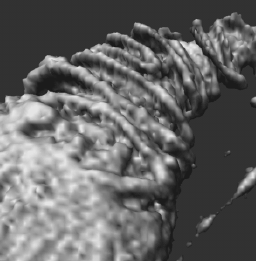
\includegraphics[width=\linewidth]{Figure7-19a}
		\caption*{$\Delta x = \Delta y = \Delta z = 1.0$}\label{fig:Figure7-19a}
	\end{subfigure}
	\hfill
	\begin{subfigure}[h]{0.48\linewidth}
		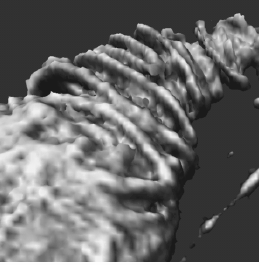
\includegraphics[width=\linewidth]{Figure7-19b}
		\caption*{$\Delta x = \Delta y = \Delta z = 2.0$}\label{fig:Figure7-19b}
	\end{subfigure}%
	\caption{A comparison of shaded images with two different step sizes used during normal estimation. Confocal microscopy data courtesy of Howard Hughes Medical Institute, SUNY Stony Brook.}\label{fig:Figure7-19}
\end{figure}


It is often the case that transfer functions based on scalar value and even gradient magnitude are not capable of fully classifying a volume. Ultrasound data is an example of particularly difficult data that does not perform well with simple segmentation techniques. While no one technique exists that is universally applicable, there exists a wide variety of techniques that produce classification information at each sample. For instance, \cite{Kikinis96} provides techniques for classifying the human brain. In order to properly handle this information a volume renderer must access the original volume and a classification volume. The classification volume usually contains material percentages for each sample, with a set of color and opacity transfer functions for each material used to define appearance.

\section{Volumetric Illumination}

The volume rendered images that we have shown so far in this chapter do not include any lighting effects. Scientist sometimes prefer to visualize their volumes using these simpler methods because they fear that adding lighting effects to the image will interfere with their interpretation. For example, in a maximum intensity projection, a dark region in the image clearly indicates the lack of high opacity values in the corresponding region of the volume, while a dark feature in a shaded image may indicate either low opacity values or values with gradient directions that point away from the light source.

\begin{figure}[!htb]
	\begin{subfigure}[h]{0.32\linewidth}
		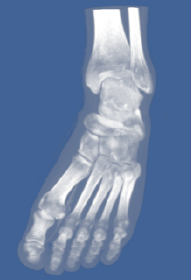
\includegraphics[width=\linewidth]{Figure7-20a}
		\caption*{Maximum intensity}\label{fig:Figure7-20a}
	\end{subfigure}
	\hfill
	\begin{subfigure}[h]{0.32\linewidth}
		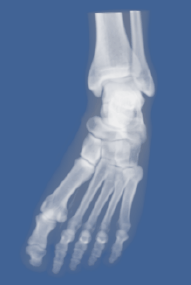
\includegraphics[width=\linewidth]{Figure7-20b}
		\caption*{Composite (unshaded)}\label{fig:Figure7-20b}
	\end{subfigure}%
	\hfill
	\begin{subfigure}[h]{0.32\linewidth}
		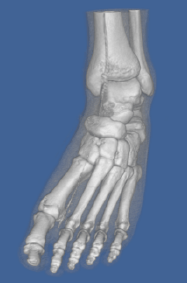
\includegraphics[width=\linewidth]{Figure7-20c}
		\caption*{Composite (shaded)}\label{fig:Figure7-20c}
	\end{subfigure}%
	\caption{A comparison of three volume rendering techniques. A maximum intensity projection does not include occlusion or shading. A composite image includes occlusion and can include shading.}\label{fig:Figure7-20}
\end{figure}

There are several advantages to lighting that can often justify the additional complexity in the image. First, consider the fact that volume rendering is a process of creating a 2D image from 3D data. The person viewing that data would like to be able to understand the 3D structure of the volume from that image. Of course, if you were to look at a photograph of a skeleton it would be easy to understand its structure from the 2D representation. The two main clues that you received from the picture are occlusion and lighting effects. If you were to view a video of the skeleton, you would receive the additional clue of motion parallax. A static image showing a maximum intensity projection does not include occlusion or lighting effects, making it difficult to understand structure. An image generated with a compositing technique does include occlusion, and the compositing ray function can be modified to include shading as well. A comparison of these three methods is shown in Figure \ref{fig:Figure7-19} for a CT scan of a human foot.

To accurately capture lighting effects, we could use a transport theory illumination model \cite{Krueger91} that describes the intensity of light $I$ arriving at a pixel by the path integral along the ray:

\begin{equation}\label{eq:7.4}
I\left(t_0, \overrightarrow{\omega\ }\right) = \bigintssss_{t_0}^{\infty} Q\left(\tau\right) e^{\left(-\bigintsss_{\ t_0}^{\ t} \sigma_\text{a}\left(\tau'\right) + \sigma_\text{sc}\left(\tau'\right) \, \text{d} \tau'\right)} \, \text{d}\tau
\end{equation}
\myequations{Path integral for light intensity.}

If we are using camera clipping planes, then $t_0$ and $\infty$ would be replaced
by the distance to the near clip plane $t_{near}$ and the distance to
the far cl[ip] $t_{far}$ respectively. The contribution $Q(t)$ from each sample at a distance $t$ along the ray is attenuated according to how much intensity is lost on the way from $t$ to $t_0$ due to absorption $\sigma_a(t')$ and scattering $\sigma_{sc}(t')$. The
contributions at $t$ can be defined as:

\begin{equation}\label{eq:7.5}
Q(t) = E(t) + \sigma_\text{sc}(t) \bigintssss_{4\pi} \rho_{sc}(\overrightarrow{\omega\ }' \to \overrightarrow{\omega\ }) I(t, \overrightarrow{\omega\ }') \, \text{d}\overrightarrow{\omega\ }'
\end{equation}
\myequations{The contribution from each sample using camera clipping planes.}

The contribution consists of the amount of light directly emitted by the sample $E(t)$, plus the amount of light coming from all directions that is scattered by this sample back along the ray. The fraction of light arriving from the $\vec{\omega'}$ direction that is scattered into the direction $\vec{\omega}$ is defined by the scattering function $\rho_{sc}(\vec{\omega'}\rightarrow \vec{\omega})$. To compute the light arriving from all directions due to multiple bounce scattering, we must recursively compute the illumination function.

If scattering is accurately modelled, then basing the ray function on the transport theory illumination model will produce images with realistic lighting effects. Unfortunately, this illumination model is too complex to evaluate, therefore approximations are necessary for a practical implementation. One of the simplest approximations is to ignore scattering completely, yielding the following intensity equation:

\begin{equation}\label{eq:7.6}
I\left(t_0, \overrightarrow{\omega\ }\right) = \bigintssss_{t_0}^{\infty} E\left(\tau\right) e^{\left(-\bigintsss_{\ t_0}^{\ t} \sigma_\text{a}\left(\tau'\right)\text{d} \tau'\right)} \, \text{d}\tau
\end{equation}
\myequations{Path integral for light intensity ignoring scattering.}

We can further simplify this equation by allowing $α(t)$ to represent both the amount of light emitted per unit length and the amount of light absorbed per unit length along the ray. The outer integral can be replaced by a summation over samples along the ray within some clipping range, while the inner integral can be approximated using an over operator:

\begin{equation}\label{eq:7.7}
I(t_\text{near}, \overrightarrow{\omega\ }) = \sum_{t\ =\ t_\text{near}}^{t\ \leq\ t_\text{far}} \alpha(t) \prod_{t'\ =\ t_\text{near}}^{t'\ <\ t}\left(1 - a(t') \right)
\end{equation}
\myequations{Simplifying Equation \ref{eq:7.6}.}

This equation is typically expressed in its recursive form:

\begin{equation}\label{eq:7.8}
I(t_n, \overrightarrow{\omega\ }) = \alpha(t_n) + \left(1 - \alpha(t_n) \right) I(t_{n + 1}, \overrightarrow{\omega\ })
\end{equation}
\myequations{The recursive form of Equation \ref{eq:7.7}.}

which is equivalent to the simple compositing method using the over operator that was described previously. Clearly in this case we have simplified the illumination model to the point that this ray function does not produce images that appear to be realistic.

If we are visualizing an isosurface within the volumetric data, then we can employ the surface illumination model described in Chapter 3 to capture ambient and diffuse lighting as well as specular highlights. There are a variety of techniques for estimating the surface normal needed to evaluate the shading equation. If the image that is produced as a result of volume rendering contains the distance from the view plane to the surface for every pixel, then we can post-process the image with a 2D gradient estimator to obtain surface normals. The gradient at some pixel $(x_p, y_p)$ can be estimated with a central difference technique by:

\begin{equation}\label{eq:7.9}
\begin{array}{lll}
\dfrac{\partial Z}{\partial x} &\simeq& \dfrac{Z\left(x_p + \Delta x, y_p\right) - Z\left(x_p - \Delta x, y_p\right)}{2 \Delta x} \\ \\
\dfrac{\partial Z}{\partial y} &\simeq& \dfrac{Z\left(x_p, y_p + \Delta y\right) - Z\left(x_p, y_p - \Delta y\right)}{2 \Delta y} \\ \\
\dfrac{\partial Z}{\partial z} &\simeq& 1
\end{array}
\end{equation}
\myequations{Estimating the gradient at $(x_p, y_p)$.}

\begin{figure}[!htb]
	\begin{subfigure}[h]{0.48\linewidth}
		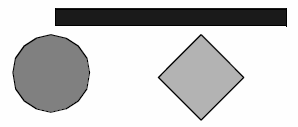
\includegraphics[width=\linewidth]{Figure7-21a}
		\caption*{Disjoint volumetric objects}\label{fig:Figure7-21a}
	\end{subfigure}
	\hfill
	\begin{subfigure}[h]{0.48\linewidth}
		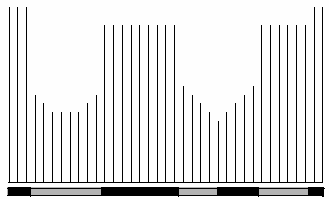
\includegraphics[width=\linewidth]{Figure7-21b}
		\captionsetup{justification=centering}
		\caption*{continuous curvature regions\\Corresponding depth image}\label{fig:Figure7-21b}
	\end{subfigure}%
	\caption{A scene (left) and the corresponding depth image (right) used in 2D gradient estimation.}\label{fig:Figure7-21}
\end{figure}

The results are normalized to produce a unit normal vector. As with the 3D finite differences gradient estimator given in Equation \ref{eq:7.3} , care must be taken when selecting $\Delta x$ and $\Delta y$. Typically these values are simply the pixel spacing in $x$ and $y$ so that neighboring pixel values are used to estimate the gradient, although larger values can be used to smooth the image.

One problem with the 2D gradient estimation technique described above is that normals are computed from depth values that may represent disjoint regions in the volume, as shown in Figure \ref{fig:Figure7-21}. This may lead to a blurring of sharp features on the edges of objects. To reduce this effect, we can locate regions of continuous curvature in the depth image, then estimate the normal for a pixel using only other pixel values that fall within the same curvature region \cite{Yagel92a}. This may require reducing our $\Delta x$ and $\Delta y$ values, or using an off-centered differences technique to estimate the components of the gradient. For example, the $x$ component of the gradient could be computed with a forward difference:

\begin{equation}\label{eq:7.10}
\dfrac{\partial Z}{\partial x} \simeq \dfrac{Z(x_p + \Delta x, y_p) - Z(x_p, y_p)}{\Delta x}
\end{equation}
\myequations{Forward difference approximation of the $x$ component.}

or a backward difference

\begin{equation}\label{eq:7.11}
\dfrac{\partial Z}{\partial x} \simeq \dfrac{Z(x_p, y_p) - Z(x_p - \Delta x, y_p)}{\Delta x}
\end{equation}
\myequations{Backward difference approximation of the $x$ component.}

Although 2D gradient estimation is not as accurate as the 3D version, it is generally faster and allows for quick lighting and surface property changes without requiring us to recompute the depth image. However, if we wish to include shading effects in an image computed with a compositing technique, we need to estimate gradients at many locations within the volume for each pixel. A 3D gradient estimation technique is more suitable for this purpose. An illumination equation for compositing could be written as:

\begin{equation}\label{eq:7.12}
I(t_\text{near}, \overrightarrow{\omega\ }) =  \sum_{t\ =\ t_\text{near}}^{t\ \leq\ t_\text{far}} \alpha(t)\left(I_\text{a} + I_\text{d} + I_\text{s}\right) \prod_{t'\ =\ t_\text{near}}^{t'\ <\ t}\left(1 - a(t') \right)
\end{equation}
\myequations{Illumination equation for compositing.}

where the ambient illumination $I_a$, the diffuse illumination $I_d$, and the specular illumination $I_s$ are computed as in surface shading using the estimated volume gradient in place of the surface normal. In this equation, $\alpha(t)$ represents the amount of light reflected per unit length along the ray, with $1 - \alpha(t)$ indicating the fraction of light transmitted per unit length.

\begin{figure}[!htb]
	\begin{subfigure}[h]{0.48\linewidth}
		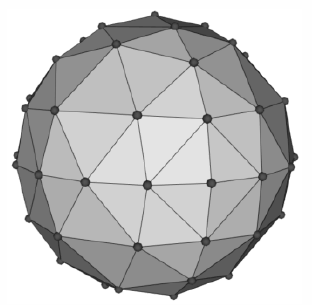
\includegraphics[width=\linewidth]{Figure7-22a}
		\caption*{Sphere at recursion level 2}\label{fig:Figure7-22a}
	\end{subfigure}
	\hfill
	\begin{subfigure}[h]{0.48\linewidth}
		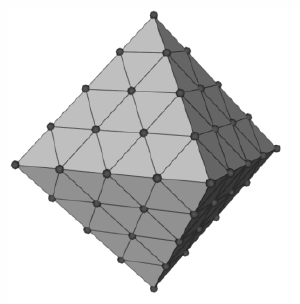
\includegraphics[width=\linewidth]{Figure7-22b}
		\caption*{Vertices pushed onto octahedron}\label{fig:Figure7-22b}
	\end{subfigure}%
	\hfill
	\begin{subfigure}[h]{0.48\linewidth}
		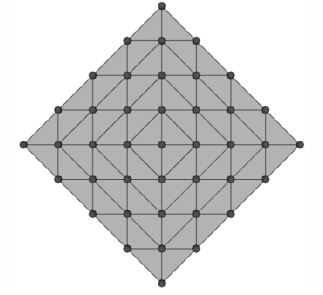
\includegraphics[width=\linewidth]{Figure7-22c}
		\caption*{Flattened onto $z = 0$ plane}\label{fig:Figure7-22c}
	\end{subfigure}%
	\hfill
	\begin{subfigure}[h]{0.48\linewidth}
		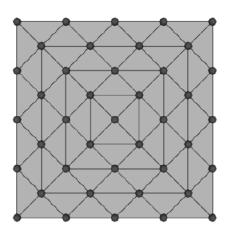
\includegraphics[width=\linewidth]{Figure7-22d}
		\caption*{Rotated 45 degrees}\label{fig:Figure7-22d}
	\end{subfigure}%
	\caption{Gradient direction encoding.}\label{fig:Figure7-22}
\end{figure}


As in classification, we have to make a decision about whether to directly compute illumination at an arbitrary location in the volume, or to compute illumination at the grid points and then interpolate. This is not a difficult decision to make on the basis of accuracy since it is clearly better to estimate the gradient at the desired location rather than interpolate from neighboring estimations. On the other hand, if we do interpolate from the grid points then we can precompute the gradients for the entire dataset once, and use this to increase rendering performance for both classification and illumination. The main problem is the amount of memory required to store the precomputed gradients. A naive implementation would store a floating-point value (typically four bytes) per component of the gradient per scalar value. For a dataset with one $256^3$ one-byte scalars, this would increase the storage requirement from 16 Mbytes to 218 Mbytes.

In order to reduce the storage requirements, we could quantize the precomputed gradients by using some number of bits to represent the magnitude of the vector, and some other number of bits to encode the direction of the vector. Quantization works well for storing the magnitude of the gradient, but does not provide a good distribution of directions if we simply divide the bits among the three components of the vector. A better solution is to use the uniform fractal subdivision of an  octahedron into a sphere as the basis of the direction encoding, as shown in Figure \ref{fig:Figure7-22}. The top left image shows the results obtained after the recursive replacement of each triangle with four new triangles, with a recursion depth of two. The vector directions encoded in this representation are all directions formed by creating a ray originating at the sphere's center and passing through a vertex of the sphere. The remaining images in this figure illustrate how these directions are mapped into an index. First we push all vertices back onto the original faces of the octahedron, then we flatten this sphere onto the plane $z=0$. Finally, we rotate the resulting grid by 45$^\circ$. We label the vertices in the grid with indices starting at 0 at the top left vertex and continue across the rows then down the columns to index 40 at the lower right vertex. These indices represent only half of the encoded normals because when we flattened the octahedron, we placed two vertices on top of each other on all but the edge locations. Thus, we can use indices 41 through 81 to represent vectors with a negative \emph{z} component. Vertices on the edges represent vectors with out a \emph{z} component, and although we could represent them with a single index, using two keeps the indexing scheme more consistent and, therefore, easier to implement.

The simple example above requires only 82 values to encode the 66 unique vector directions. If we use an unsigned short to store the encoded direction, then we can use a recursion depth of 6 when generating the vertices. This leads to 16,642 indices representing 16,386 unique directions.

Once the gradients have been encoded for our volume, we need only compute the illumination once for each possible index and store the results in a table. Since data samples with the same encoded gradient direction may have different colors, this illumination value represents the portion of the shading equation that is independent of color. Each scalar value may have separate colors defined for ambient, diffuse, and specular illumination; therefore, the precomputed illumination is typically an array of values.

Although using a shading table leads to faster rendering times, there are some limitations to this method. Only infinite light sources can be supported accurately since positional light sources would result in different light vectors for data samples with the same gradient due to their different positions in the volume. In addition, specular highlights are only captured accurately for orthographic viewing directions where the view vector does not vary based on sample position. In practice, positional light sources are often approximated by infinite light sources, and a single view direction is used for computing specular highlights since the need for fast rendering often outweighs the need for accurate illumination.

\section{Regions of Interest}

\section{3D Widgets and User Interaction}
\label{sec:3dwui}

Chapter 3: \nameref{chap:computer_graphics_primer} provided an introduction to interaction techniques for graphics (see ``Introducing vtkRenderWindowInteractor'' on page \pageref{pg:rwi} ).
In the context of visualization, interaction is an essential feature of systems that provide methods for data exploration and query. The classes
vtkRenderWindowInteractor and vtkInteractorStyle are core constructs used in VTK to capturewindowing-system specific events in the render window, translate them into VTK events, and then take action as appropriate to that event invocation.
In Chapter 3: \nameref{chap:computer_graphics_primer} we saw how these classes could be used to manipulate the camera and actors to interactively produce a desired view. This functionality, however, is relatively limited in its ability to interact with data. For example, users often wish tointeractively control the positioning of streamline starting points, control the orientation of a clipping plane, or transform an actor. While using interpreted languages (see ``Interpreted Code'' on page \pageref{pg:rwi} ) can go a long way to provide this interaction, in some situations the ability to see what you are doing when placing objects is essential. Therefore, it is apparent that a variety of user interaction techniques is required by the visualization system if it is to successfully support real-world applications.

\section{Chapter Summary}

Alpha opacity is a graphics method to simulate transparent objects. Compositing is the process of blending translucent samples in order. Alpha compositing requires the data to be ordered properly.

Texture mapping is a powerful technique to introduce additional detail into an image without extensive geometric modelling. Applying 2D texture maps to the surface of an object is analogous to pasting a picture. The location of the texture map is specified via texture coordinates.

Volume rendering is a powerful rendering technique to view the interior of inhomogeneous objects. Most volume rendering techniques can be classified as image-order or object-order, although some are a combination of the two while others do not fall into either category. Object-order techniques generally composite voxels in front-to-back or back-to-front order. Image-order techniques cast rays through pixels in the image plane to sample the volume. Other methods may traverse both the image and the volume at the same time or may operate in the frequency domain.

For effective visualization of volumetric data, classification and shading are important considerations. Regions of interest may be used to reduce the amount of data visible in an image. Due to the complexity of volume rendering algorithms, efficiency and methods that allow for interactivity are critical.

Stereo rendering techniques create two separate views for the right and left eyes. This simulates binocular parallax and allows us to see depth in the image. Time multiplexed techniques alternate left and right eye views in rapid succession. Time parallel techniques display both images at the same time.

Raster devices often suffer from aliasing effects. Antialiasing techniques are used to minimize the effects of aliasing. These techniques create blended images that soften the boundary of hard edges.

By using an accumulation buffer we can create interesting effects, including motion blur and focal blur. In motion blurring we accumulate multiple renders as the actors move. To simulate focal blur, we jitter the camera position and hold its focal point constant.

Effective visualizations are inherently interactive. Not only are camera manipulation models required for different types of data, but methods to interact, query, and modify data are essential. 3D widgets are important contributions to this end. They provide intuitive graphical interface to the data through a representation in the scene that can be easily manipulated. 3D widgets also generate supplemental information such as implicit functions, output polygonal data, and transformation matrices that may be applied to objects in the scene.

\section{Bibliographic Notes}

An overview of volume rendering and volume visualization techniques can be found in a tutorial by Kaufman \cite{Kaufman91}. Many of the volume rendering techniques discussed in this chapter are also accessible from research institutions as source code. The shear-warp algorithm is provided within the VolPack rendering library and is available on the Web at \href{http:www-graphics.stanford.edu/software/volpack/}{VolPack} . SUNY Stony Brook offers a turnkey volume visualization system called VolVis to nonprofit and government organizations. Source code and executable versions are available at \href{http://www.cs.sunysb.edu/\~volvis}{VolVis}. In addition, an application called Vis5D is available that applies volume visualization techniques to time varying atmospheric weather data. Vis5D may be obtained from the Web location \href{http://vis5d.sourceforge.net}{Vis5D}. A commercial volume rendering application, VolView, developed on top of The Visualization Toolkit, is available from Kitware for a 30-day trial at \href{http://www.kitware.com/products/volview.html}{VolView}.

\printbibliography


\section{Exercises}

\begin{itemize}

\item In astronomy, photographs can be taken that show the movements of the stars over a period of time by keeping the camera's shutter open. Without accounting for the rotation of the earth, these photographs display a swirl of circular arcs all centered about a common point. Such time lapse photography is essentially capturing motion blur. If we tried to simulate these images using the motion blur technique described in this chapter, they would look different from the photographs. Why is this? How could you change the simple motion blur algorithm to correct this?

\item In Figure \ref{fig:Figure7-25} we show the difference between stereo rendering with two or one view planes. If you were viewing a rectangle head-on (its surface normal parallel to your direction), what artifacts would be introduced by rendering onto one view plane while using the equations for two planes

\item On some graphics systems transparent objects are rendered using a technique called screen door transparency. Basically, every pixel is either completely opaque or completely transparent. Any value in between is approximated using dithering. So a polygon that was 50 percent opaque would be rendered by drawing only half of the pixels. What visual artifacts does this introduce? What blending problems can arise in using such a technique?

\item In this chapter we describe a few different techniques for anti--aliased rendering. One technique involved rendering a large image and then scaling it down to the desired size using bilinear interpolation. Another technique involved rendering multiple images at the desired size using small camera movements and then accumulating them into a final image. When rendering a model with a surface representation, these two techniques will produce roughly the same result. When rendering a model with a wireframe representation there will be significant differences. Why is this?

\item You need to create a small image of a volume dataset to include on your web page. The dataset contains $512^3$ voxels and the desired image size is$100^2$ pixels. You can use a software object-order method that projects each voxel onto the image, or a software ray casting method that casts one ray for each pixel. Assuming that identical images are created, which method would you select, and why?

\item Two software developers implement volume rendering methods. The first developer uses a software ray casting approach, while the second uses a graphics hardware texture mapping approach. The grayscale images are generated and displayed on a workstation with an 8 bit frame buffer (256 levels of gray). They both use the same interpolation method and the same compositing scheme, yet the two methods produce different images even though the same number of samples from identical locations were used to generate the images. Why is this?

\item In the classification of some medical dataset, scalar values from 100 to 200 represent skin, 200 to 300 represent muscle and 300 to 400 represent bone. The color transfer functions define skin as tan, muscle as red, and bone as white. If we interpolate scalar value and then perform classification, what classification artifacts may appear in the image?

\item The normal encoding example illustrated in Figure \ref{fig:Figure7-22} produced 82 indices at a recursion depth of two, which would require seven bits of storage. If we instead use a recursion depth of three, how many indices are there? How many unique vector directions does this represent? How many bits of storage does this require?

\item Writing an object-order back-to-front projection algorithm is more difficult for a perspective viewing transformation than a parallel viewing transformation. Explain why this is and draw a 2D diagram of the volume and the viewing frustum that illustrates the issues.

\end{itemize}
